\documentclass{article}

\usepackage[utf8]{inputenc}
\usepackage[T1]{fontenc}
\usepackage[spanish]{babel}
\usepackage{times}
\usepackage{wrapfig}
\usepackage{lmodern}
\usepackage{mathtools}
\usepackage{graphicx}
\usepackage[utf8]{inputenc}
\usepackage{color}
\usepackage{hyperref}
\usepackage{fancyhdr,lipsum}


\hypersetup{
    colorlinks=true, %set true if you want colored links
    linktoc=all,     %set to all if you want both sections and subsections linked
    linkcolor=blue,  %choose some color if you want links to stand out
}
\urlstyle{same}

\title{PRACTICA TEMA 2}
\author{Antonio Muñoz Cubero}
\date{12 de Noviembre de 2020}

\begin{document}
  \maketitle
  \pagenumbering{gobble}
  \pagestyle{fancy}
  
  \newpage
    \tableofcontents
    \lhead[PRACTICA TEMA 2]{PRACTICA TEMA 2}
    \lfoot[IES Francisco De Los Rios]{IES Francisco De Los Rios}

  \newpage
    \section{Enunciado}
    
    Tenemos que copiar  el  código del archivo adjunto, que este caso, muestro en la imagen inferior.
    \begin{itemize}      
      \item Compilar el programa y corregir los errores sintácticos. Incluyendo las librerías que sean necesarias.
      \item Realizar la depuración y posterior ejecución del programa.
      \item Personalizar la configuración del IDE, creando una configuración nueva, llamada \textbf{miconfiguración} para ese proyecto de la siguiente manera: 
      El directorio de trabajo será una carpeta llamada \textit{DirectorioTrabajoED}, que estará situada en el escritorio.
      \item Tras ello, desinstalar los plugins instalados anteriormente.
      \item Actualizar todos los complementos del IDE (si no hay nada que actualizar pon la captura de la pantalla donde se indica).
    \end{itemize}

    \begin{figure}[h]
      \centering
      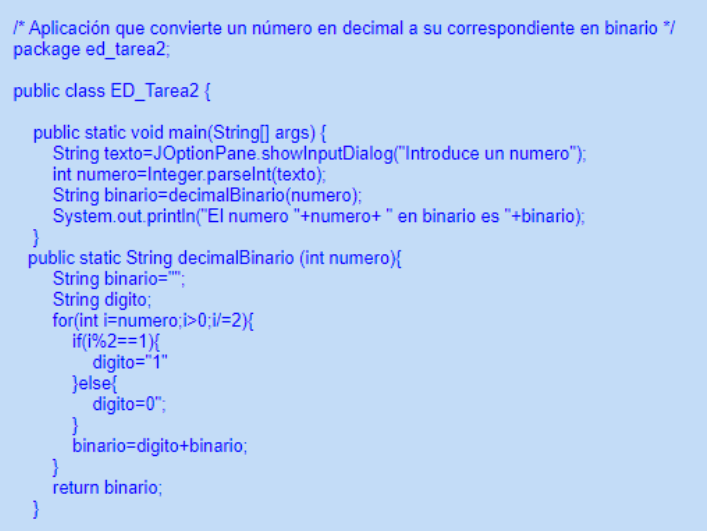
\includegraphics[scale = 0.5]{img/codigo.png}
    \end{figure}


\end{document}